\documentclass[tikz]{standalone}
\usepackage{wasysym}
\usepackage{SIunits}
\usepackage{pgfplots}
\pgfplotsset{compat=1.5}
\usetikzlibrary{plotmarks,arrows}
\tikzset{>=latex}
\definecolor{tissueColour}{RGB}{251,185,130}
\definecolor{lesionColour}{RGB}{175,50,53}
\begin{document}
	\begin{tikzpicture}[x=0.038\textwidth, y=0.038\textwidth, draw=black, text=black, fill=black]
		% the main domain area
		\draw[fill=tissueColour] (0, 0) rectangle(4, 10);

		% the lesion
		%\draw (2, 3) node{
\includegraphics[width=0.076\textwidth]{images/blob_colour.png}};
		\draw (2, 3) node{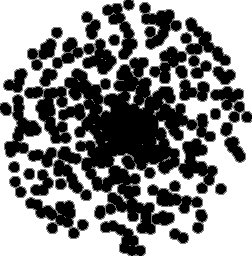
\includegraphics[width=0.076\textwidth]{images/blob.png}};

		% lesion size
		\draw (2, 3) circle(1);
		\draw[<-] (1.293, 2.293) -- (0.5, 1) -- (1, 1) node[right]{\scriptsize $\diameter S$};

		% blob size
		\draw[<-] (1.85, 3.38) -- (2.75, 4.5) node[right]{\scriptsize $r_{bl}$};

	\end{tikzpicture}
\end{document}